\section{How it works}
\label{sec:barcode_functioning}

In barcodes, black and white stripes encode data visually. For certain types of codes, they represent 1s and 0s, while for other types such as Code-39, it is the width of the stripes which determines the value. The following sections will explain more thoroughly some of the most used types of barcodes.

\subsection{Code-39}
\label{ssec:code39}

First of all, there is Code-39, one of the simplest type of barcode. It can encode 43 different alphanumerical characters plus the special '*' delimiter. Each character is assigned a particular group of 9 bits, 3 of which are 1s, hence the name. Table \ref{tab:code39} lists all encodable characters and their respective codes.

\def\arraystretch{1.5}
\begin{table}[H]
  \centering
  \begin{tabu}{|[2pt]c|c|[2pt]c|c|[2pt]c|c|[2pt]}
    \tabucline[2pt]{-}
    Char & Code & Char & Code & Char & Code \\
    \tabucline[2pt]{-}
    A & 100001001 & P & 001010010 & 4 & 000110001 \\
    \hline
    B & 001001001 & Q & 000000111 & 5 & 100110000 \\
    \hline
    C & 101001000 & R & 100000110 & 6 & 001110000 \\
    \hline
    D & 000011001 & S & 001000110 & 7 & 000100101 \\
    \hline
    E & 100011000 & T & 000010110 & 8 & 100100100 \\
    \hline
    F & 001011000 & U & 110000001 & 9 & 001100100 \\
    \hline
    G & 000001101 & V & 011000001 & \emph{space} & 011000100 \\
    \hline
    H & 100001100 & W & 111000000 & - & 010000101 \\
    \hline
    I & 001001100 & X & 010010001 & \$ & 010101000 \\
    \hline
    J & 000011100 & Y & 110010000 & \% & 000101010 \\
    \hline
    K & 100000011 & Z & 011010000 & . & 110000100 \\
    \hline
    L & 001000011 & 0 & 000110100 & / & 010100010 \\
    \hline
    M & 101000010 & 1 & 100100001 & + & 010001010 \\
    \hline
    N & 000010011 & 2 & 001100001 & * & 010010100 \\
    \hline
    O & 100010010 & 3 & 101100000 &  &  \\
    \tabucline[2pt]{-}
  \end{tabu}
  \caption{Code-39 characters}
  \label{tab:code39}
\end{table}
\def\arraystretch{1}

To create a Code-39 barcode, we just have to take the codes corresponding to each character and join them end to end, adding a 0 in between each group. Finally, we add the '*' character at both ends (also spaced by a 0). It is a delimiter and should always be present at the beginning and end of the code, to signal scanners that it is a Code-39 barcode, as well as providing a reference for the normal bar width.

Ones represent wide bars and zeros thin bars\footnote{The ratio wide/thin must be comprised between 2:1 and 3:1 \cite{ISO16388}}. Black and white stripes alternate, starting with black.

Let's encode the string "CODE-39"

\def\arraystretch{1.5}
\begin{table}[H]
  \centering
  \begin{tabu}{|[2pt]c|c|[2pt]}
    \tabucline[2pt]{-}
    Char & Code \\
    \tabucline[2pt]{-}
    * & 010010100 \\
    \hline
    C & 101001000 \\
    \hline
    O & 100010010 \\
    \hline
    D & 000011001 \\
    \hline
    E & 100011000 \\
    \hline
    - & 010000101 \\
    \hline
    3 & 101100000 \\
    \hline
    9 & 001100100 \\
    \hline
    * & 010010100 \\
    \tabucline[2pt]{-}
  \end{tabu}
  \caption{Code-39 for "*CODE-39*"}
  \label{tab:code39_ex_codes}
\end{table}
\def\arraystretch{1}

For example, the first delimiter is encoded as:
\begin{center}
  %\begin{tabular}{p{10pt}p{10pt}p{10pt}p{10pt}p{10pt}p{10pt}p{10pt}p{10pt}p{10pt}p{10pt}p{10pt}p{10pt}}
  %\bbar & & & \bbar & & \bbar & \bbar & & \bbar & \bbar & & \bbar \\
  %0 & \multicolumn{2}{c}{1} & 0 & 0 & \multicolumn{2}{c}{1} & 0 & \multicolumn{2}{c}{1} & 0 & 0 \\
  \begin{tabular}{C{10pt}C{20pt}C{10pt}C{10pt}C{20pt}C{10pt}C{20pt}C{10pt}C{10pt}}
    \bbar & & \bbar & & \bbar & & \bbar & & \bbar \\
    0 & 1 & 0 & 0 & 1 & 0 & 1 & 0 & 0 \\
  \end{tabular}
\end{center}

The entire barcode would look like figure \ref{fig:code_39_ex}

\begin{figure}[H]
  \centering
  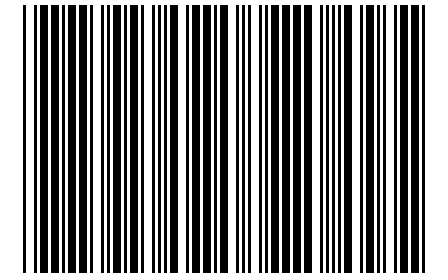
\includegraphics[width=0.5\linewidth]{images/code_39_example}
  \caption{Code-39 example ("\texttt{*CODE-39*}")}
  \label{fig:code_39_ex}
\end{figure}

Code-39 doesn't provide any error detection mechanism. If a character is read as another character, the reading device won't know that it made a mistake. Additionally, it is not the most compact type of encoding, but it can easily be used for small amounts of data, for example to encode the identification number on students' absence booklet or sheet.

\subsection{EAN}
\label{ssec:ean}

Another barcode type is the EAN\footnote{European Article Numbering} standard. It is used for product identification and can be found on anything bought from a store. It exists in two main formats: EAN-8 and EAN-13, encoding respectively 7 and 12 digits. EAN codes use what is called a check digit to detect erroneous readings. This digit is the result of the Luhn Formula. Say we want to encode the number \texttt{978294062105}. To find the checksum digit, we have to multiply each digit by the alternating factors 1 and 3, and add all the products.

\def\arraystretch{1.5}
\begin{table}[H]
  \centering
  \begin{tabu}{c|c|c|c|c|c|c|c|c|c|c|c|c|c}
    %\hline
      & 9 & 7 & 8 & 2 & 9 & 4 & 0 & 6 & 2 & 1 & 0 & 5 & \\
    %\hline
    x & 1 & 3 & 1 & 3 & 1 & 3 & 1 & 3 & 1 & 3 & 1 & 3 & \\
    \tabucline[2pt]{-}
    + & 9 &21 & 8 & 6 & 9 &12 & 0 &18 & 2 & 3 & 0 &15 & = 103 \\
    %\hline
  \end{tabu}
  \caption{Luhn Formula}
  \label{tab:luhn}
\end{table}
\def\arraystretch{1}

We then take the modulo ten, which is the same as saying we keep the unit's digit, and subtract it from $10$. In our example, $103 \equiv 3\ (\textrm{mod}\ 10)$ so the checksum is $10 - 3 = 7$. If we get $10$ we change it to $0$ to keep a single digit.

This is now the 13th digit of our code. For an EAN-8 code, the process is the same with the factors 1 and 3 inverted, meaning the first digit is multiplied by 3, the second by 1, etc.

The barcode itself is built out of a series of "elements".
Each element encodes a character, as described by table \ref{tab:ean_elmts}.
Ones are black stripes and zeros are white.

\def\arraystretch{1.5}
\begin{table}[h]
  \centering
  \begin{tabu}{|[2pt]c|c|c|c|[2pt]}
    \tabucline[2pt]{-}
    Char. & A & B & C \\
    \tabucline[2pt]{-}
    0 & 0001101 & 0100111 & 1110010 \\
    \hline
    1 & 0011001 & 0110011 & 1100110 \\
    \hline
    2 & 0010011 & 0110011 & 1101100 \\
    \hline
    3 & 0111101 & 0110011 & 1000010 \\
    \hline
    4 & 0100011 & 0110011 & 1011100 \\
    \hline
    5 & 0110001 & 0110011 & 1001110 \\
    \hline
    6 & 0101111 & 0110011 & 1010000 \\
    \hline
    7 & 0111011 & 0110011 & 1000100 \\
    \hline
    8 & 0110111 & 0110011 & 1001000 \\
    \hline
    9 & 0001011 & 0110011 & 1110100 \\
    \tabucline[2pt]{-}
  \end{tabu}
  \caption{EAN elements}
  \label{tab:ean_elmts}
\end{table}
\def\arraystretch{1}

There are 3 types of elements: A, B and C. Type C is obtained by swapping 1s and 0s from type A. Type B is obtained by flipping type C from left to right.
\begin{comment}
For example:
\def\arraystretch{1.5}
\begin{table}[h]
\centering
\begin{tabu}{|[2pt]c|c|c|c|[2pt]}
\tabucline[2pt]{-}
Char. & A & B & C \\
\tabucline[2pt]{-}
0 & 0001101 & 0100111 & 1110010 \\
\hline
1 & 0011001 & 0110011 & 1100110 \\
\tabucline[2pt]{-}
\end{tabu}
\caption{Example of EAN elements}
\label{tab:ean_elmt_ex}
\end{table}
\def\arraystretch{1}
\end{comment}

This structure makes it easy to find the type of a certain element.
Bs and Cs have an even number of 1s, while As have an odd number. Additionally, As an Bs start with 0 and end with 1, whereas Cs are the opposite.

In this way, if the code is read in the wrong way, C elements will appear as Bs, and A elements will be invalid because no element starts with a 1 and has an odd number of 1s. Similarly, if the barcode is printed with inverted colors (white on black), A elements will be read as Cs, and B elements will be invalid, since no element starts with a 1 and has an odd number of 1s.

EAN barcodes are thus very practical since they can be scanned in any orientation and support color inversion.

\subsubsection{EAN-8}
\label{sss:ean8}
An EAN-8 barcode has the following structure:
\def\arraystretch{1.5}
\begin{table}[H]
  \centering
  \begin{tabu}{|[2pt]c|c|c|c|c|c|c|c|c|c|c|[2pt]}
    \tabucline[2pt]{-}
    left & A & A & A & A & mid & C & C & C & C & right\\
    \tabucline[2pt]{-}
  \end{tabu}
  \caption{EAN-8 structure}
  \label{tab:ean8_struct}
\end{table}
\def\arraystretch{1}

In table \ref{tab:ean8_struct}, "left" and "right" are the end delimiters "101". "mid" is the center delimiter "01010".
To illustrate, let's encode the value "8427372".

\begin{enumerate}
  \item Calculate the checksum digit:
  \def\arraystretch{1.5}
  \begin{table}[H]
    \centering
    \begin{tabu}{c|c|c|c|c|c|c|c|c}
      %\hline
        & 8 & 4 & 2 & 7 & 3 & 7 & 2 & \\
      %\hline
      x & 3 & 1 & 3 & 1 & 3 & 1 & 3 & \\
      \tabucline[2pt]{-}
      + &24 & 4 & 6 & 7 & 9 & 7 & 6 & = 63 \\
      %\hline
    \end{tabu}
    \caption{Luhn Formula (EAN-8 example)}
    \label{tab:luhn_ean8_ex}
  \end{table}
  \def\arraystretch{1}

  Thus the last digit is $10 - (63 \textrm{ mod } 10) = 10 - 3 = 7$.

  %\item Take the corresponding element for each digit (As for the first 4, Cs for the last 4)
  \item Take each digit's corresponding element: As for the first 4, Cs for the rest (table \ref{tab:ean8_elmt_ex}).

  \item Add the delimiters "101" at each end and "01010" between both halves of the code.
  \item For each 1, draw a black bar and for each 0 a white one (figure \ref{fig:ean8_ex}).
\end{enumerate}

\begin{minipage}[b]{\textwidth}
  \centering
  \begin{minipage}[c]{0.26\linewidth}
    \centering
    \def\arraystretch{1.5}
    \begin{tabu}{|[2pt]c|c|[2pt]}
      \tabucline[2pt]{-}
      Char. & Element \\
      \tabucline[2pt]{-}
      8 & 0110111 \\
      \hline
      4 & 0100011 \\
      \hline
      2 & 0010011 \\
      \hline
      7 & 0111011 \\
      \tabucline[1pt]{-}
      3 & 1000010 \\
      \hline
      7 & 1000100 \\
      \hline
      2 & 1101100 \\
      \hline
      7 & 1000100 \\
      \tabucline[2pt]{-}
    \end{tabu}
    \def\arraystretch{1}
    \captionof{table}{EAN-8 example elements}
    \label{tab:ean8_elmt_ex}
  \end{minipage}
  \hfill
  \begin{minipage}[c]{0.7\linewidth}
    \centering
    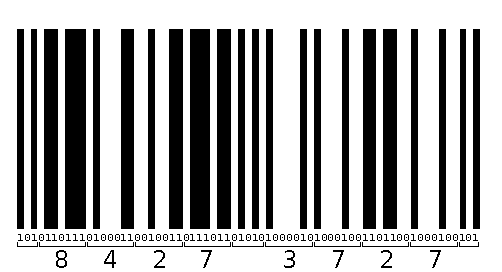
\includegraphics[width=\linewidth]{images/ean8_example_2}
    \captionof{figure}{EAN-8 example ("\texttt{84273727}")}
    \label{fig:ean8_ex}
  \end{minipage}
\end{minipage}

\subsubsection{EAN-13}
\label{sss:ean13}

EAN-13 follows the same principles as EAN-8. The structure of such a code is the following:

\def\arraystretch{1.5}
\begin{table}[H]
  \centering
  \begin{tabu}{|[2pt]c|c|c|c|c|c|c|c|c|c|c|c|c|c|c|[2pt]}
    \tabucline[2pt]{-}
    \multirow{2}{*}{left} & A & A & A & A & A & A & \multirow{2}{*}{mid} & \multirow{2}{*}{C} & \multirow{2}{*}{C} & \multirow{2}{*}{C} & \multirow{2}{*}{C} & \multirow{2}{*}{C} & \multirow{2}{*}{C} & \multirow{2}{*}{right}\\
    \cline{2-7}
    & B & B & B & B & B & B & & & & & & & & \\
    \tabucline[2pt]{-}
  \end{tabu}
  \caption{EAN-13 structure}
  \label{tab:ean13_struct}
\end{table}
\def\arraystretch{1}

This has only 12 places for elements, 6 A/B and 6 C. The 13th digit (in reality the first) is encoded in the pattern of A and B elements. Here is the list of patterns corresponding to each digit:

\def\arraystretch{1.5}
\begin{table}[H]
  \centering
  \begin{tabu}{|[2pt]c|c|[2pt]c|c|[2pt]}
    \tabucline[2pt]{-}
    Digit & Pattern & Digit & Pattern\\
    \tabucline[2pt]{-}
    0 & AAAAAA & 5 & ABBAAB \\
    \hline
    1 & AABABB & 6 & ABBBAA \\
    \hline
    2 & AABBAB & 7 & ABABAB \\
    \hline
    3 & AABBBA & 8 & ABABBA \\
    \hline
    4 & ABAABB & 9 & ABBABA \\
    \tabucline[2pt]{-}
  \end{tabu}
  \caption{EAN-13 1st digit patterns}
  \label{tab:ean13_patterns}
\end{table}
\def\arraystretch{1}

It can be noticed that the first element is always an A so that reading direction can easily be determined.

Let's illustrate EAN-13 by encoding the value "978294062105".


\begin{enumerate}
  \item Calculate the checksum digit:
  \def\arraystretch{1.5}
  \begin{table}[H]
    \centering
    \begin{tabu}{c|c|c|c|c|c|c|c|c|c|c|c|c|c}
      %\hline
        & 9 & 7 & 8 & 2 & 9 & 4 & 0 & 6 & 2 & 1 & 0 & 5 & \\
      %\hline
      x & 1 & 3 & 1 & 3 & 1 & 3 & 1 & 3 & 1 & 3 & 1 & 3 & \\
      \tabucline[2pt]{-}
      + & 9 &21 & 8 & 6 & 9 &12 & 0 &18 & 2 & 3 & 0 &15 & = 103 \\
      %\hline
    \end{tabu}
    \caption{Luhn Formula (EAN-13 example)}
    \label{tab:luhn_ean13_ex}
  \end{table}
  \def\arraystretch{1}

  Thus the last digit is $10 - (103 \textrm{ mod } 10) = 10 - 3 = 7$.

  \item Get the pattern corresponding to the first digit: 9 $\rightarrow$ ABBABA

  \item Take the corresponding element for each digit
  \def\arraystretch{1.5}
  \begin{table}[H]
    \centering
    \begin{tabu}{|[2pt]c|c|c|[2pt]|[2pt]c|c|c|[2pt]}
      \tabucline[2pt]{-}
      Char. & Type & Element & Char. & Type & Element \\
      \tabucline[2pt]{-}
      7 & A & 0111011 & 6 & C & 1010000\\
      \hline
      8 & B & 0001001 & 2 & C & 1101100\\
      \hline
      2 & B & 0011011 & 1 & C & 1100110\\
      \hline
      9 & A & 0001011 & 0 & C & 1110010\\
      \hline
      4 & B & 0011101 & 5 & C & 1001110\\
      \hline
      0 & A & 0001101 & 7 & C & 1000100\\
      \tabucline[2pt]{-}
    \end{tabu}
    \caption{EAN-13 example elements}
    \label{tab:ean13_elmt_ex}
  \end{table}
  \def\arraystretch{1}

  \item Add the delimiters "101" at each end and "01010" between both halves of the code.
  \item For each 1, draw a black bar and for each 0 a white one.

  \begin{figure}[H]
    \centering
    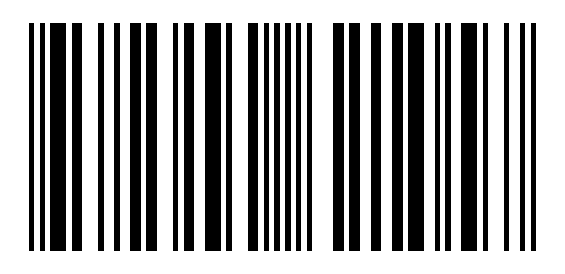
\includegraphics[width=0.5\linewidth]{images/ean13_example}
    \caption{EAN-13 example ("\texttt{9782940621057}")}
    \label{fig:ean13_ex}
  \end{figure}
\end{enumerate}
